\chapter{Planos}

\section{Equação geral do plano}

Seja $A$ um ponto de um plano $\pi$ e $\vec n$ um vetor não nulo ortogonal a $\pi$. Um ponto $P$ pertence a $\pi$ se os vetores $\vec n$ e $\overrightarrow{AP}$ são ortogonais, isto é, $\vec n \cdot \overrightarrow{AP}=0$.

\begin{multicols}{2}
\begin{figure}[H]
\centering
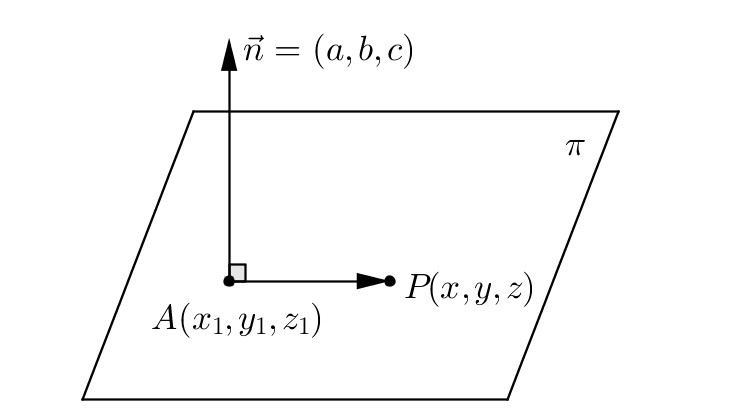
\includegraphics[scale=1]{analitica/imagens/plano.png}
\end{figure}

$$\pi: ax + by + cz + d = 0$$

\end{multicols}


\section{Equação vetorial do plano}

Sejam $A$ um ponto de um plano $\pi$ e, $\vec u$ e $\vec v$ são dois vetores não colineares paralelos a $\pi$. Se o ponto $P$ pertence ao plano $\pi$ então existem dois números reais $h$ e $t$, tais que $\overrightarrow{AP}=h\vec u+t\vec v$ ou $P=A+h\vec u+t\vec v$.

\begin{multicols}{2}
\begin{figure}[H]
\centering
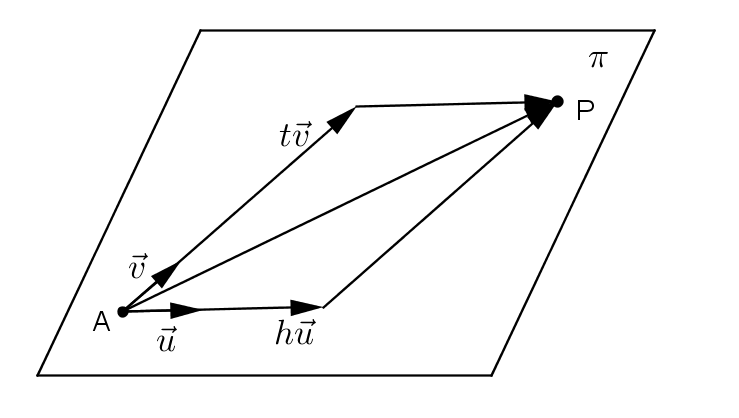
\includegraphics[scale=1]{analitica/imagens/plano-vet.png}
\end{figure}

$(x,y,z)=(x_1,y_1,z_1)+h(a_1,b_1,c_1)+t(a_2,b_2,c_2)$
\end{multicols}

\section{Equações paramétricas do plano}

Da equação vetorial do plano, vem:

$$\left\{ \begin{array}{l}
x=x_1+a_1h+a_2t\\
y=y_1+b_1h+b_2t\\
z=z_1+c_1h+c_2t \end{array} \right. $$

\section{Planos paralelos aos eixos coordenados}

\begin{enumerate}[(a)]
 \item Se um plano $\pi$ é paralelo ao eixo $Ox$, o seu vetor normal $\vec n$ é ortogonal ao vetor $\vec i$, e  portanto $\vec n=(0,b,c)$. Neste caso, a equação de $\pi$  tem a forma $by + cz + d = 0$.
 \item Se um plano $\pi$ é paralelo ao eixo $Oy$, o seu vetor normal $\vec n$ é ortogonal ao vetor $\vec j$, e  portanto, $\vec n=(a,0,c)$. Neste caso, a equação de $\pi$ tem a forma $ax+cz+d=0$.
 \item Se um plano $\pi$ é paralelo ao eixo $Oz$, o seu vetor normal $\vec n$ é ortogonal ao vetor $\vec k$, e portanto, $\vec n=(a,b,0)$. Neste caso, a equação de $\pi$ tem a forma $ax+by+d=0$.
\end{enumerate}

\textbf{Importante:} Se uma das componentes do vetor normal é nula, o plano é paralelo ao eixo correspondente a componente nula (a variável ausente na equação, indica o eixo ao qual o plano é paralelo).

\section{Planos paralelos aos planos coordenados}

\begin{enumerate}[(a)]
 \item Se um plano $\pi$ é paralelo ao plano $xOy$, qualquer vetor normal $\vec n$ tem a direção do vetor $\vec k$, e portanto, $\vec n=(0,0,c)$. Neste caso, a equação de $\pi$ tem a forma $cz+d=0$.
 \item Se um plano $\pi$ é paralelo ao plano $xOz$, qualquer vetor normal $\vec n$ tem a  direção do vetor $\vec j$,e portanto, $\vec n=(0,b,0)$. Neste caso, a equação de $\pi$ tem a forma $by+d=0$.
 \item Se um plano $\pi$ é paralelo ao plano $yOz$, qualquer vetor normal $\vec n$ tem a direção do vetor $\vec i$, e portanto, $\vec n=(a,0,0)$. Neste caso, a equação de $\pi$ tem a forma $ax+d=0$.
\end{enumerate}

\textbf{Importante:} Se duas componentes do vetor normal forem nulas, o plano é  paralelo ao plano correspondente as componentes nulas (as variáveis ausentes na equação, indicam o plano coordenado ao qual o plano é paralelo).

\section{Ângulo de dois planos}

O ângulo entre dois planos $\pi_1$ e $\pi_2$ é a medida do ângulo entre duas retas $r_1$ e $r_2$, respectivamente, perpendiculares a $\pi_1$ e $\pi_2$.

\begin{multicols}{2}
\begin{figure}[H]
\centering
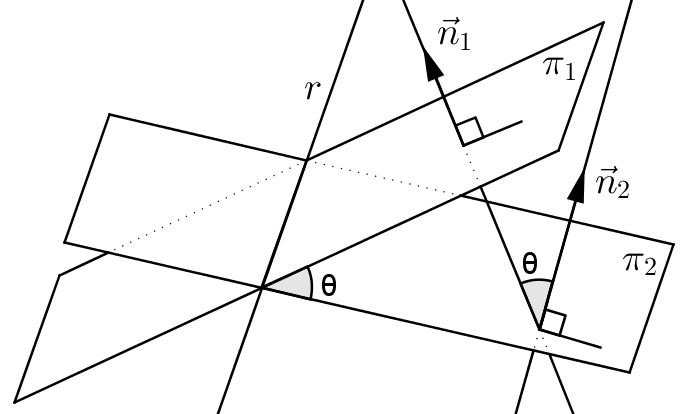
\includegraphics[scale=1]{analitica/imagens/planos-ang.png}
\end{figure}

$$\cos{\theta}=\frac{|\vec n_1 \cdot \vec n_2|}{\Vert \vec n_1 \Vert \Vert \vec n_2 \Vert} \qquad 0\leq \theta \leq \frac{\pi}{2}$$

\end{multicols}

$\pi_1\parallel \pi_2 \quad\Longleftrightarrow \quad \vec n_1 \parallel \vec n_2$

$\pi_1\perp \pi_2 \quad\Longleftrightarrow \quad \vec n_1 \perp \vec n_2$

\section{Intersecção de dois planos}

\begin{multicols}{2}
\begin{figure}[H]
\centering
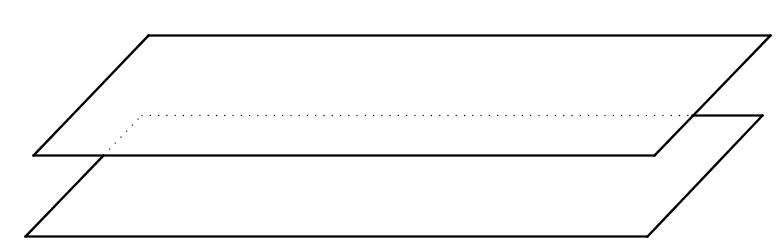
\includegraphics[scale=1]{analitica/imagens/planos-par.png}
\end{figure}

\noindent Planos paralelos não possuem intersecção.

\end{multicols}

\begin{multicols}{2}
\begin{figure}[H]
\centering
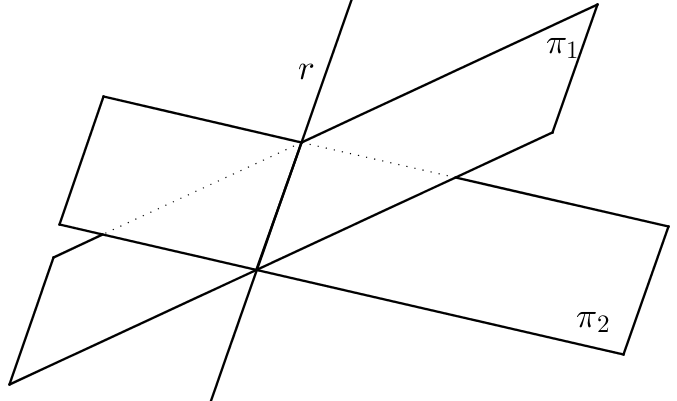
\includegraphics[scale=1]{analitica/imagens/planos-inter.png}
\end{figure}

\noindent A intersecção dos planos $\pi_1$ e $\pi_2$ é a reta $r$ cujas equações são obtidas resolvendo-se o sistema formado pelas equações de $\pi_1$ e $\pi_2$.

$$\left\{ \begin{array}{l} \pi_1: a_1x+b_1y+c_1z+d_1=0\\   \pi_2: a_2x+b_2y+c_2z+d_2=0 \end{array} \right.$$


\end{multicols}




\textbf{Observação:} Sejam $\left\{ \begin{array}{l} y=mx+n\\   z=px+q \end{array} \right.$ as equações reduzidas da reta $r$, intersecção dos planos $\pi_1$ e $\pi_2$. Cada equação de $r$ pode ser obtida através da  eliminação no sistema acima da variável ausente na equação.

\section{Ângulo de uma reta com um plano}

O ângulo $\phi$, da reta $r$ com o plano é o complementar do ângulo entre a reta $r$ e uma reta $s$ perpendicular a $\pi$, com $0\leq \phi \leq \frac{\pi}{2}$.


\begin{multicols}{2}
\begin{figure}[H]
\centering
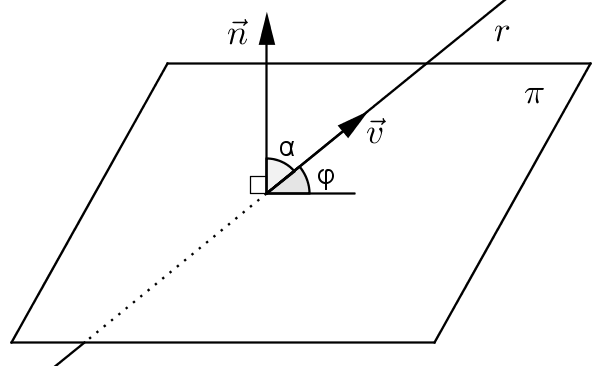
\includegraphics[scale=1]{analitica/imagens/plano-reta-a.png}
\end{figure}

$$\cos{\alpha}=\frac{|\vec v \cdot \vec n|}{\Vert \vec v \Vert \Vert \vec n \Vert}$$

$$\phi=\frac{\pi}{2}-\alpha$$

\end{multicols}




\section{Intersecção de reta com plano}

\begin{multicols}{2}
\begin{figure}[H]
\centering
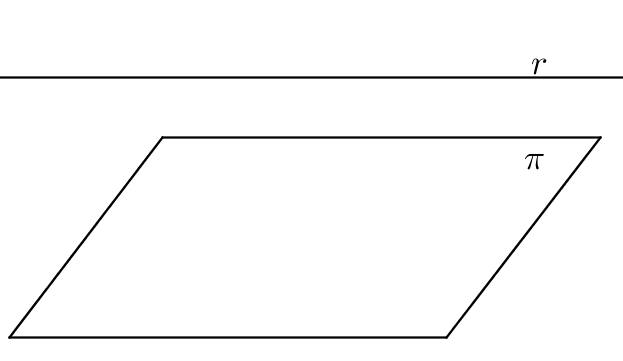
\includegraphics[scale=1]{analitica/imagens/plano-reta2.png}
\end{figure}

\noindent Quando a reta $r$ for paralela ao plano $\pi$, então não haverá interseção entre reta e plano. Neste caso, o sistema formado pelas equações da reta $r$ e do plano $\pi$ não possuirá solução.
\end{multicols}

\begin{multicols}{2}
\begin{figure}[H]
\centering
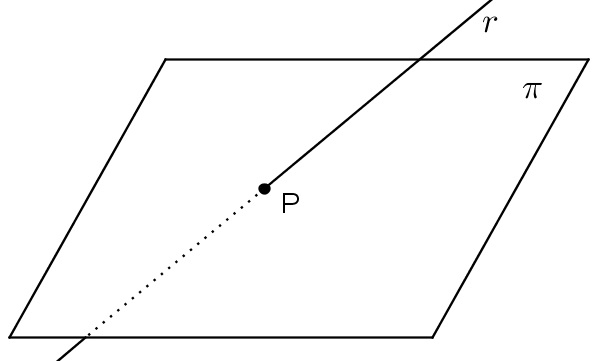
\includegraphics[scale=1]{analitica/imagens/plano-reta.png}
\end{figure}

\noindent Quando a reta $r$ for concorrente ao plano $\pi$, então a intersecção entre plano e reta será um ponto $P$. As coordenadas deste ponto são obtidas com a solução do sistema formado pelas equações da reta $r$ e do plano $\pi$.
\end{multicols}

Há ainda a situação em que a reta $r$ está contida no plano, e neste caso, todos os pontos da reta estarão no plano. Neste caso, o sistema formado pelas equações da reta $r$ e do plano $\pi$ será considerado indeterminado, pois possuirá infinitas soluções.